%
% Niniejszy plik stanowi przykład formatowania pracy magisterskiej na
% Wydziale MIM UW.  Szkielet użytych poleceń można wykorzystywać do
% woli, np. formatujac wlasna prace.
%
% Zawartosc merytoryczna stanowi oryginalnosiagniecie
% naukowosciowe Marcina Wolinskiego.  Wszelkie prawa zastrzeżone.
%
% Copyright (c) 2001 by Marcin Woliński <M.Wolinski@gust.org.pl>
% Poprawki spowodowane zmianami przepisów - Marcin Szczuka, 1.10.2004
% Poprawki spowodowane zmianami przepisow i ujednolicenie
% - Seweryn Karłowicz, 05.05.2006
% Dodanie wielu autorów i tłumaczenia na angielski - Kuba Pochrybniak, 29.11.2016

% dodaj opcję [licencjacka] dla pracy licencjackiej
% dodaj opcję [en] dla wersji angielskiej (mogą być obie: [licencjacka,en])
\documentclass[licencjacka]{pracamgr}

%\autor{Autor Zerowy}{342007}
\autori{Paweł Giżka}{TODO}
\autorii{Szymon Gajda}{TODO}
\autoriii{Kamil Ćwintal}{TODO}
\autoriv{Tomasz Kanas}{385674}
%\autorv{Autor nr Pięć}{342011}

\title{Mobilna aplikacja do dzielenia się żywnością ``Podziel się''}


%\tytulang{An implementation of a difference blabalizer based on the theory of $\sigma$ -- $\rho$ phetors}

%kierunek:
% - matematyka, informacyka, ...
% - Mathematics, Computer Science, ...
\kierunek{informatyka}

% informatyka - nie okreslamy zakresu (opcja zakomentowana)
% matematyka - zakres moze pozostac nieokreslony,
% a jesli ma byc okreslony dla pracy mgr,
% to przyjmuje jedna z wartosci:
% {metod matematycznych w finansach}
% {metod matematycznych w ubezpieczeniach}
% {matematyki stosowanej}
% {nauczania matematyki}
% Dla pracy licencjackiej mamy natomiast
% mozliwosc wpisania takiej wartosci zakresu:
% {Jednoczesnych Studiow Ekonomiczno--Matematycznych}

% \zakres{Tu wpisac, jesli trzeba, jedna z opcji podanych wyzej}

% Praca wykonana pod kierunkiem:
% (podać tytuł/stopień imię i nazwisko opiekuna
% Instytut
% ew. Wydział ew. Uczelnia (jeżeli nie MIM UW))
\opiekun{dra Janusza Jabłonowskiego\\
  Instytut Informatyki\\
  }

% miesiąc i~rok:
\date{Czerwiec 2019}

%Podać dziedzinę wg klasyfikacji Socrates-Erasmus:
\dziedzina{
%11.0 Matematyka, Informatyka:\\
%11.1 Matematyka\\
%11.2 Statystyka\\
11.3 Informatyka\\
%11.4 Sztuczna inteligencja\\
%11.5 Nauki aktuarialne\\
%11.9 Inne nauki matematyczne i informatyczne
}

%Klasyfikacja tematyczna wedlug AMS (matematyka) lub ACM (informatyka)
\klasyfikacja{D. Software\\
}

% Słowa kluczowe:
\keywords{aplikacja mobilna, żywność, ReactNative}

% Tu jest dobre miejsce na Twoje własne makra i~środowiska:
\newtheorem{defi}{Definicja}[section]
\usepackage{hyperref}
\usepackage{graphicx}

% koniec definicji

\begin{document}

\maketitle

%tu idzie streszczenie na strone poczatkowa
\begin{abstract}
\textit{``Podziel się''} to aplikacja mobilna przeznaczona do wzajemnego dzielenia się żywnością dla użytkowników systemów operacyjnych Android oraz iOS\@. Celem projektu było stworzenie platformy, która umożliwi łatwe i bezpłatne dzielenie się jedzeniem z innymi mieszkańcami w okolicy: osoby posiadające nadwyżkę artykułów żywnościowych lub gotowych potraw mogą przekazać je użytkownikom, którzy zadeklarują chęć ich odbioru. W niniejszej pracy przedstawiono szczegółowy opis aplikacji i jej architektury, oraz przybliżono proces jej powstawania.
\end{abstract}

\tableofcontents
%\listoffigures
%\listoftables

\chapter*{Wprowadzenie}
\addcontentsline{toc}{chapter}{Wprowadzenie}
\section*{Problematyka}
Obecnie w Polsce istnieją liczne grupy entuzjastów wymiany żywności funkcjonujące na portalach społecznościowych (przeważnie na Facebooku), jednak duża liczebność tych grup uniemożliwia skuteczną organizację wymiany jedzenia w satysfakcjonujący sposób. Aplikacja \textit{``Podziel się''} będzie wspierać dalsze funkcjonowanie tej inicjatywy oraz zapewni zwolennikom idei food sharingu platformę do efektywnej wymiany żywności, także w znacznie większej skali.

\section*{Kontekst społeczny}
Według współczesnych szacunków (\cite{fao}), około 1/3 wytworzonej na świecie żywności nigdy nie zostanie zjedzona. Skala problemu jest szczególnie widoczna w danych Eurostatu, z których wynika, że w Polsce marnuje się około 9 milionów ton żywności rocznie. Jej wartość sięga około 50 złotych miesięcznie w przeliczeniu na~jednego mieszkańca Polski. Badanie Millward Brown wykazało, że do wyrzucania jedzenia przyznaje się 35\% Polaków, podczas gdy wyrzucane produkty mogłyby przyczynić się do zaspokojenia podstawowych potrzeb żywieniowych niemal 3 mln osób żyjących w skrajnym ubóstwie. Nasz kraj jest piątym wśród państw Unii Europejskiej, w których marnuje się najwięcej żywności.

W krajach rozwiniętych około 50\% wyrzucanego jedzenia pochodzi z gospodarstw domowych, w których na skutek nierozważnego planowania zakupów jedzenie ulega zepsuciu i~trafia do śmietnika. Wierzymy, że~możliwe jest przeciwdziałanie temu zjawisku na poziomie lokalnym.

Istnieją ruchy społeczne (dumpster diving, freeganizm, zero waste) promujące możliwie racjonalny obrót żywnością oraz uwrażliwiające społeczeństwo na problem masowego wyrzucania jedzenia.

\section*{Zamawiający}
Aplikacja \textit{``Podziel się''} powstała na zamówienie pani Marii Skołożyńskiej, działaczki społecznej oraz pomysłodawczyni akcji \textit{Podziel się Posiłkiem z Bezdomnymi}, podczas której mieszkańcy całej Polski mogą przekazać pozostałe po świętach (Bożego Narodzenia, Wielkanocy) posiłki do wolontariuszy, którzy zajmują się transportem jedzenia do osób potrzebujących. Pani Maria jest wolontariuszką działającą na rzecz przeciwdziałania marnowaniu jedzenia oraz główną koordynatorką akcji dystrybucji żywności. Działalność pani Marii Skołożyńskiej ma zasięg ogólnopolski; akcje gromadzenia żywności dla bezdomnych i ubogich działają obecnie w kilkudziesięciu miastach, m.\ in.\ w Warszawie, Krakowie, Wrocławiu, Trójmieście, Szczecinie, Toruniu, Bydgoszczy, Katowicach, Łodzi. W 2018 r.\ akcja \textit{Podziel się Posiłkiem z Bezdomnymi}, w~uznaniu dla skuteczności działania oraz promocji pozytywnych postaw społecznych, otrzymała Europejską Nagrodę Reduce Food Waste.

\section*{Osoby zaangażowane w projekt}
Aplikacja \textit{``Podziel się''} została opracowana oraz wdrożona przez zespół studentów informatyki Uniwersytetu Warszawskiego: Kamila Ćwintala, Szymona Gajdę, Pawła Giżkę oraz Tomasza Kanasa. Opiekę nad projektem sprawował dr Janusz Jabłonowski. Wymagania funkcjonalne zostały dostarczone zespołowi przez pomysłodawczynie projektu: p. Marię Skołożyńską oraz p. Martynę Dakowską.

\section*{Grupa docelowa}
Aplikacja \textit{``Podziel się''} jest przeznaczona dla użytkowników smartfonów, którym nie jest obojętny problem marnowania żywności. \textit{``Podziel się''} może stanowić interesującą propozycję dla osób, które nie mają czasu na przygotowanie posiłku albo gotują zbyt dużo (i~jednocześnie nie chcą wyrzucać nadwyżki jedzenia). Aplikacja \textit{``Podziel się''} zrzesza społeczność osób zainteresowanych tematyką food sharingu i zero waste, które dbają o środowisko naturalne oraz racjonalną gospodarkę żywnością.

\section*{Opis funkcjonalności}
Aplikacja \textit{``Podziel się''} umożliwia:
\begin{itemize}
\setlength\itemsep{-0.2em}
\item bezpłatną rejestrację nowego konta,
\item uzupełnienie własnego profilu o podstawowe dane personalne,
\item dodawanie nowego ogłoszenia (opisu produktu wraz z preferowaną lokalizacją miejsca odbioru),
\item zamieszczenie w ogłoszeniu zdjęć produktu, opakowania, etykiet itp.,
\item przeglądanie dostępnych do odebrania posiłków w okolicy aktualnej lokalizacji użytkownika,
\item sortowanie dostępnych ogłoszeń w oparciu o wprowadzone przez użytkownika kryteria i preferencje,
\item funkcję czatu między odbiorcą a darczyńcą w celu ustalenia szczegółów odbioru, zadawania pytań,
\item przechowywanie historii konwersacji z innymi użytkownikami,
\item wskazanie użytkownika (ze zbiorczej listy osób zainteresowanych ogłoszeniem), która otrzyma wystawiony~produkt/artykuł żywnościowy,
\item pośrednictwo w procesie przekazania żywności,
%TODO czy to jest zrobione? chyba tak
\item usuwanie ogłoszeń zrealizowanych pomyślnie lub ogłoszeń, dla których minęła data przydatności do~spożycia,
\item system recenzji/ocen użytkowników,
%TODO tego nie ma nie?
\item oznaczanie wybranych użytkowników jako ``obserwowanych'', dzięki czemu ich nowe ogłoszenia będą dodatkowo eksponowane na liście dostępnych ogłoszeń,
%TODO czy to jest zrobione?
\item flagowanie ogłoszeń o nieodpowiedniej zawartości, co skutkuje powiadomieniem moderatora o~konieczności~weryfikacji zamieszczonej treści,
\end{itemize}
Aplikację wyróżnia nowoczesny interfejs graficzny, zaprojektowany specjalnie na potrzeby projektu.

\section*{Zawartość pracy}
W rozdziale~\ref{r:konkurencja} przedstawiono przegląd i analizę konkurencyjnych rozwiązań. Rozdział~\ref{r:arch} zawiera opis użytych technologi i architektury systemu. W kolejnych rozdziałach opisano implementację aplikacji i wybrane przypadki użycia. Rozdział~\ref{r:problem} opisuje problemy i trudności które napotkaliśmy podczas tworzenia aplikacji oraz jak sobie z nim poradziliśmy. Ostatnie rozdziały zawierają instrukcje budowania aplikacji i zawartość płytki dołączonej do pracy, podział pracy w zespole i krótkie podsumowanie pracy.

\chapter{Przegląd konkurencyjnych rozwiązań}\label{r:konkurencja}

\section{Sytuacja na rynku}
Od paru lat można zaobserwować ciągły wzrost zainteresowania tematyką marnowania żywności wśród społeczeństwa. Przejawia się to na przykład w rosnącym zainteresowaniu polityków i władz, w tym Komisji Europejskiej (patrz~\cite{ec}), bardzo licznym publikacjom na ten temat, a także w rosnącej popularności ruchów społecznych takich ``freeganizm'', czy ``zero waste''. Zainteresowanie tym tematem przejawia się też w licznych aplikacjach pomagających wymieniać się jedzeniem które inaczej by się zmarnowało. Co ciekawe w różnych państwach popularne są różne aplikacje. Na przykład w Wielkiej Brytanii najpopularniejsze jest \textit{Olio}, w Zachodniej Europie \textit{Too Good To Go}, a w Stanach Zjednoczonych ``Unsung''. W Polsce nie ma jeszcze żadnej popularnej aplikacji, chociaż funkcjonują grupy na portalach społecznościowych spełniające podobną funkcję. W dalszej części tego rozdziału zostaną dokładniej omówione wybrane z konkurencyjnych rozwiązań.

\section{Olio}
Z wymienionych w tym rozdziale aplikacji \textit{Olio} jest najbardziej podobne do \textit{Podziel Się}. Posiada bardzo prosty interfejs, pozwalający już kilka chwil po zainstalowaniu dodać swoje pierwsze ogłoszenie, czy znaleźć z listy ogłoszeń (która może być sortowana po odległości, lub czasie dodania ogłoszenia) produkt na który mamy ochotę. \textit{Olio} tak samo jak \textit{Podziel Się} jest zintegrowane z Mapami Google i lokalizacją telefonu (choć można ją wyłączyć). \textit{Olio} posiada też proste forum, które uznaliśmy za zbędne w takiej aplikacji, nie posiada natomiast podziału ogłoszeń na kategorie (np.\ wegańskie, bezglutenowe itp.), w \textit{Olio} specyfikuje się tylko czy produkt jest żywnością czy nie.

\textit{Olio} jest bardzo popularną aplikacją. Na chwilę obecną posiada ponad milion użytkowników i ponad półtora miliona ogłoszeń (\cite{olio}). Jest najbardziej popularna w Wielkiej Brytanii, w Polsce praktycznie nie funkcjonuje.

\section{Too Good To Go}
Ta aplikacja reprezentuje zupełnie inne podejście niż \textit{Podziel Się}. Służy do umożliwienia restauracjom i jadłodajnią do odsprzedania niesprzedanych posiłków po znacznie niższych cenach niedługo przed zamknięciem. Oznacza, to że oferty są zwykle płatne, w przeciwieństwie do \textit{Podziel Się}, gdzie wszystkie oferty są darmowe. \textit{Too Good To Go} ma trochę bardziej skomplikowany interfejs niż \textit{Olio}, czy Podziel się. Tak jak poprzednie aplikacje jest zintegrowana z Mapami Google i lokalizacją telefonu, umożliwia też przeglądanie mapy z zaznaczonymi wszystkimi dostępnymi jadłodajniami, oraz dodawania jadłodajni do listy swoich ulubionych.

\textit{Too Good To Go} jest popularna w praktycznie całej Zachodniej Europie, posiadając obecnie prawie 25.000 współpracujących jadłodajni (\cite{tgtg}). W Warszawie jest tylko \~20 jadłodajni.

\section{Grupa ``Freeganism, dumpster diving, food sharing --- Warszawa''}
Jest to grupa funkcjonująca na portalu społecznościowym Facebook. Nie jest to co prawda aplikacja, jednak służy do tego samego celu i jest największą lokalną konkurencją. Grup tego rodzaju jest wiele zarówno w Polsce jak i w samej Warszawie, ta została wybrana jako przykładowa głównie ze względu na największą popularność, ponieważ w chwili obecnej liczy prawie 9 tysięcy członków i publikowanych na niej jest około 700 postów miesięcznie. Główny problem takich grup wynika z niedostosowania platformy --- portalu Facebook. Nie posiada on narzędzi umożliwiających wygodne przeglądanie listy aktualnych ofert, nie pozwala filtrować, ani sortować ogłoszeń po odległości, ani nawet łatwo odfiltrować już wygasłe ogłoszenia. Bardzo ogranicza to rozrost takich grup. Z ciekawych rozwiązań z których ta grupa korzysta jest koncept jadłodzielni. Są to zwykle ogólnodostępne lodówki i szafki na żywność w których można umieszczać produkty których się nie spożyje. Udostępniane są one zwykle przez różne jednostki jak: urząd miasta, uniwersytet, czy centrum kultury. Jest to szczególnie wygodne w odbiorze, ponieważ nie trzeba nawet wiedzieć, że ktoś ma coś do oddania, wystarczy jak się jest w pobliżu sprawdzić, czy nie ma w niej akurat czegoś na co ma się ochotę.

\chapter{Implementacja}\label{r:arch}

\section{Architektóra systemu}
Architektóra aplikacji \textit{``Podziel się''} składa się z dwóch głównych komponentów: aplikacji mobilnej oraz części serwerowej. Wykorzystywane są również zewnętrzne usługi takie jak Firebase, Facebook, GoogleMaps, AmazonS3.

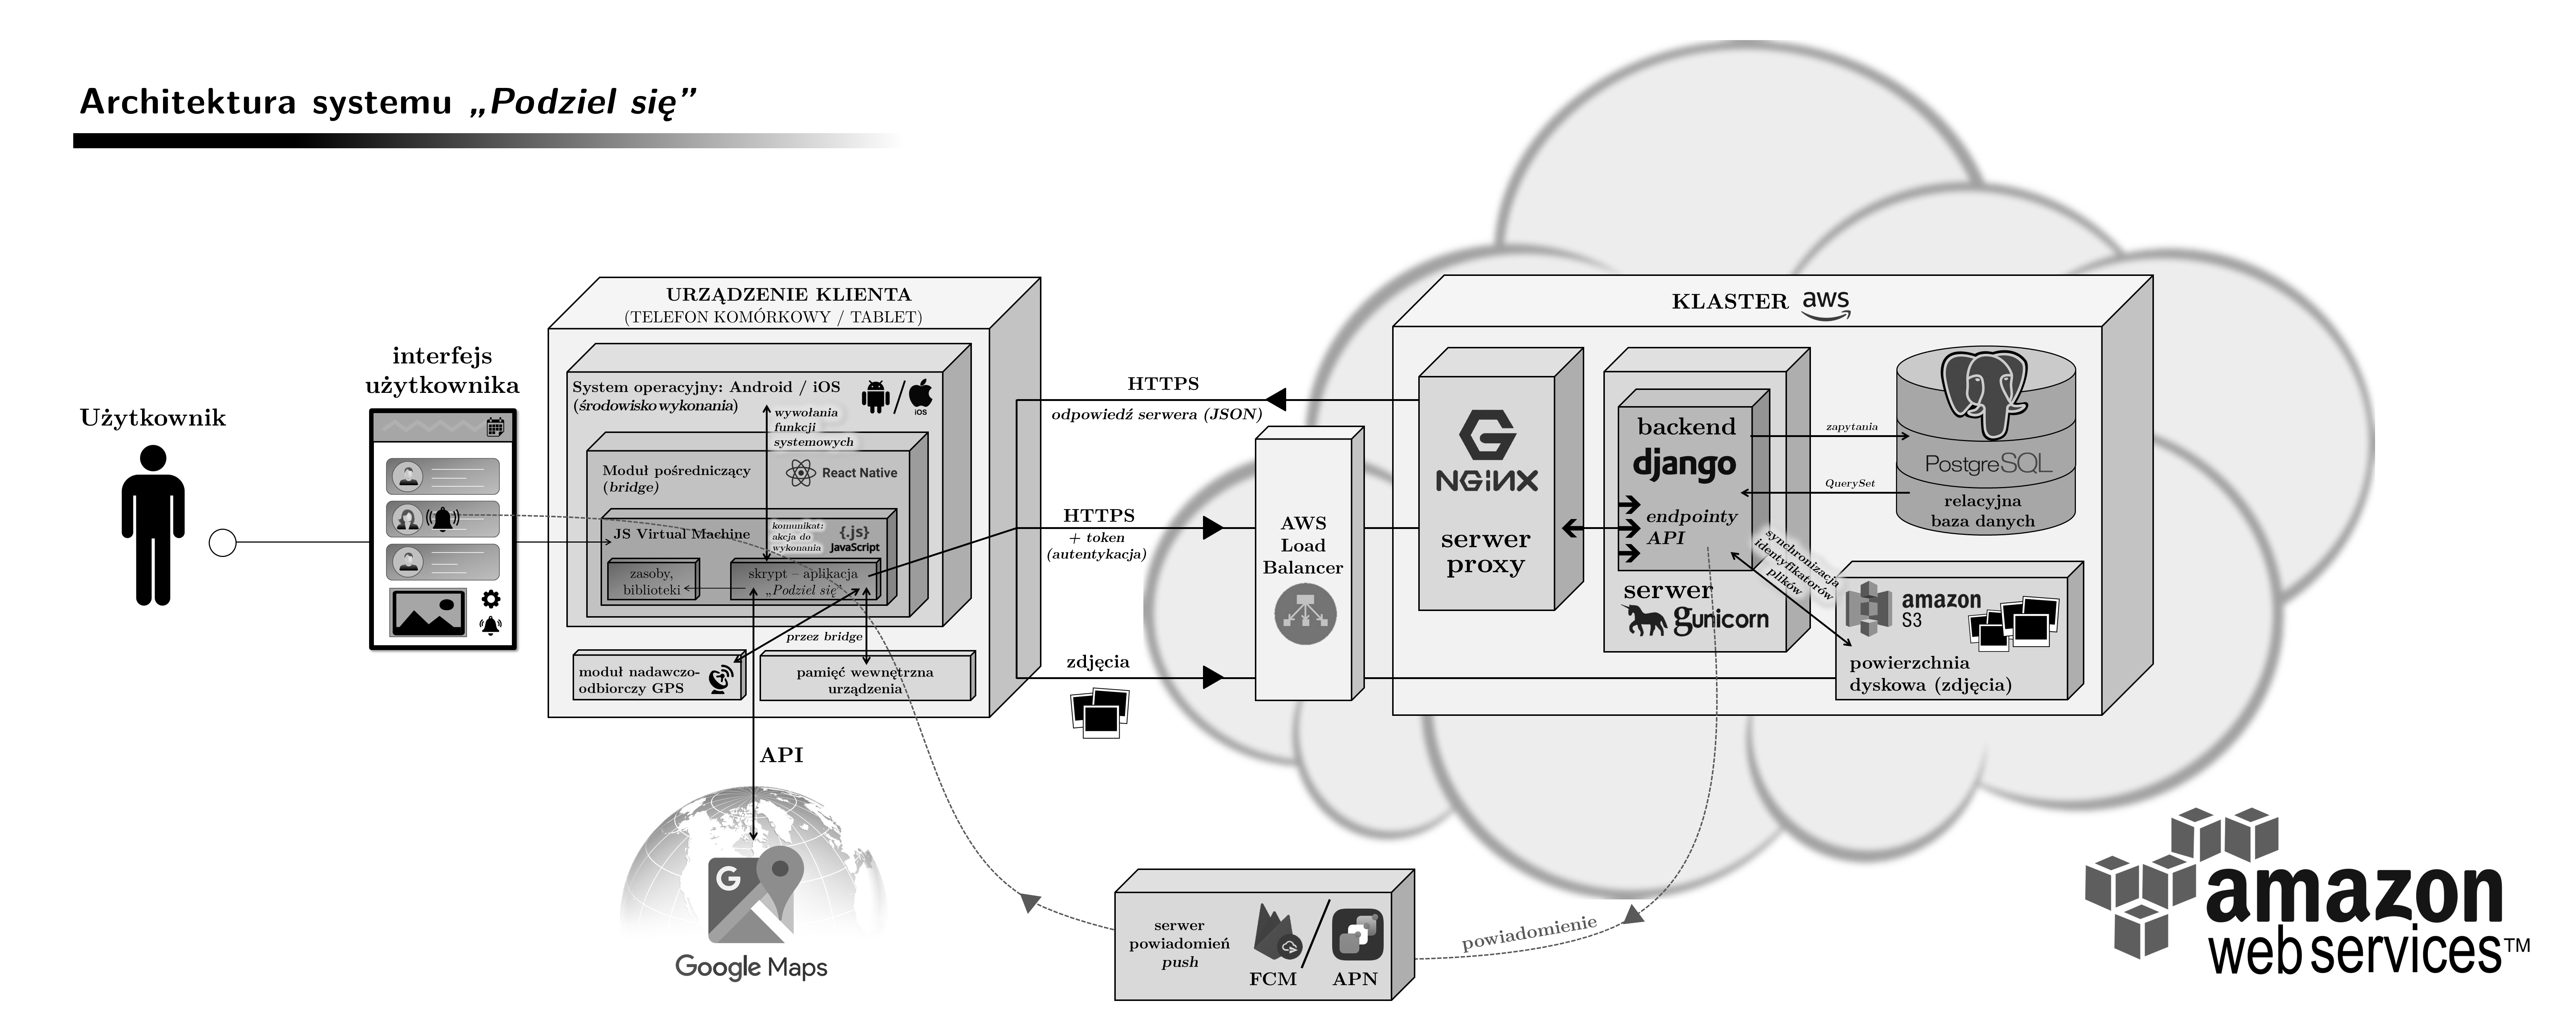
\includegraphics[width=\linewidth]{architektura.png}

\subsection{Aplikacja mobilna}
Aplikacja \textit{``Podziel się''} przeznaczona jest dla użytkowników dwóch najpopularniejszych mobilnych systemów operacyjnych: Androida oraz iOS\@. Interfejs aplikacji powstał z wykorzystaniem nowoczesnego frameworka React Native, pozwalającego opisać graficzne rozmieszczenie elementów na ekranie w składni zbliżonej do arkuszy stylów CSS, zaś logikę działania aplikacji w kodzie JavaScriptu. W React Native, przy użyciu specjalnego języka znaczników JSX, zostały zdefiniowane tzw.\ komponenty (lista ogłoszeń, przycisk wysyłania wiadomości, menu szufladkowe, okienko z komunikatem itp.), na bazie których React Native buduje komponenty natywne dla Androida oraz iOS\@. Pozwala to na ujednolicenie wyglądu interfejsu graficznego dla użytkowników różnych systemów i architektur --- aplikacja nie odbiega wyglądem od rozwiązań natywnych, projektowanych specjalnie z myślą~o~konkretnej platformie. Filozofia React Native polega na stosowaniu schematów tworzenia aplikacji webowych przy projektowaniu aplikacji działających w środowisku mobilnym, w szczególności możliwe jest korzystanie z rozmaitych pomocniczych bibliotek JavaScriptu.


Ważnym elementem React Native jest moduł pośredniczący (ang. \textit{bridge}), który tłumaczy wywołania pochodzące z wątków JavaScriptu na polecenia skierowane do systemu operacyjnego. Komunikaty opisujące akcje do wykonania są przesyłane w formacie JSON do modułu pośredniczącego, a po ich otrzymaniu \textit{bridge} wywołuje odpowiednie funkcje systemowe. Wymiana komunikatów jest asynchroniczna oraz nieblokująca, zatem React Native nie ingeruje nadmiernie w pracę systemu operacyjnego oraz umożliwia sprawne renderowanie widoków na ekranie. Co więcej, aplikacja ma możliwość swobodnej komunikacji ze środowiskiem wykonania; w razie potrzeby może uzyskać dostęp do modułu GPS, aparatu, pamięci wewnętrznej urządzenia itp.

\subsection{Część Serwerowa} 

Cześć serwerowa została stworza w języku Python, w oparciu o framework Django. Pozwala on na szybkie tworzenie webowych interfejsów programistycznych aplikacji (po angielsku Web API) oraz łatwy dostęp do relacyjnych baz danych dzięki rozbudowanemu mechanizmowi mapowania obiektowo-relacyjnego (ORM). Polega ono na odwzorowaniu logicznych modeli encji, reprezentowanych jako klasy w języku Python, na rzeczywistą treść skryptów tworzących tabele i więzy spójności w bazie danych. Podobnie, wyniki zapytań są konwertowane do obiektu typu QuerySet, który może podlegać dalszemu przetwarzaniu przez serwer.

Jednym z głównych wymogów zamawiającej było stworzenie panelu administracyjnego. Wybrany framework umożliwa automatyczne generowanie panelu administratora. Wygenerowany panel umożliwia wykonywanie podstawowych operacji: pobierz, dodaj, usuń, modyfikuj na danych znajdujących się w bazie. 

%Nie wiedziałem jak napisać to zdanie: 
Do przychowywania danych wykorzystana została relacyjna baza danych PostegreSql z wtyczką PostGIS, która pozwala na wydajne wykonywanie zapytań zapytań przestrzennych. Zdjęcia zapisywane są w usłudze AmazonS3.

\subsection{Komunikacja Klient - Serwer} 
Wymiana danych pomiędzy aplikacją mobilną a serwerem odbywa się za pomocą bezstanowego protokołu HTTP. Dane przesyłana są w formacie JSON, jest on formatem tekstowym i bazuje na podzbiorze języka JavaScript. Każde zapytanie do serwera uwierzytelniane jest unikalnym tokenem przyznwanym w momencie logowania bądź rejestracji, w związku z tym hasło użytkownika nie jest przechowywane w pamięci telefonu. Przy każdym ponownym logowaniu generowany jest nowy token. 

Dane z serwera do urządzenia mobilnego (powiadomienia) wysyłane są natomiast za pośrednictwem usługi Firebase.

\section{Postgis}
%liczenie odległosci itd.

\section{Przechowywanie zdjęć} 
%tutaj pasowało by napisać dlaczego nie składowanie danych na dysku

Projekt wykorzystuje usługę pokrewną firmy Amazon, Amazon Simple Storage Service (Amazon S3) do przechowywania zdjęć użytkowników aplikacji w sposób trwały i bezpieczny. Zaletą Amazon S3 jest nieograniczona pojemność dyskowa oraz brak narzuconych limitów na transfer wychodzący; koszt usługi jest proporcjonalny do sumarycznego rozmiaru przechowywanych danych. Transfer plików z platformy hostingowej jest szyfrowany protokołem SSL, ponadto same dane podlegają 256-bitowemu szyfrowaniu po stronie serwera.

W dalszej perspektywie, w miarę rozwoju projektu, Amazon S3 oferuje rozszerzone plany wykorzystania oraz opcję archiwizacji danych z możliwością łatwego odtworzenia w przypadku nadpisania, usunięcia lub utracenia plików.

\section{Powiadomienia}
%tutaj dlaczego nie odpytywanie serwera non stop co jakiś czas

Aplikacja \textit{``Podziel się''} wspiera użytkowników w zarządzaniu licznymi ogłoszeniami wykorzystując mechaniz powiadomień. Wspomniana funkcjonalność pozwala na wyświetlanie użytkownikom krótkich komunikatów o zajściu zdarzeń wymagających uwagi.

Powiadomienia wyświetlane są w przypadku zajaścia jednego z następujących zdarzeń:
\begin{itemize}
\setlength\itemsep{-0.2em}
    \item otrzymanie wiadomości od innego użytkownika,
    \item dodanie nowego ogłoszenia w okolicy,
    \item dodanie nowego ogłoszenia przez obserwowaną osobę
    \item polubienie naszego ogłoszenia,
\end{itemize}{}

Najprostszym sposobem implementacji tej funkcjonalności jest regularne odpytywanie serwera czy są dostępne nowe powiadomienia. Jednakże ze względu na ograniczenia systemu Android jak i IOS, obsługa procesów w tle (to znaczy wtedy kiedy użytkownik nie korzysta z aplikacji) jest bardzo mocno ograniczona. Procesy w tle nie mogą być uruchamiane częściej niż co kilkadziesięt minut. Związane jest to z oszcządzaniem energi.

Z tego względu zdecydowaliśmy się na użycie zewnętrznych usług takich jak: Firabase Cloud Messaging (FCM), dla systemu Androida oraz Apple Push Notification (APN) w przypadku IOS. Umożliwiają one niemalże natychmiastowe dostarczanie wiadomości z serwera do telefonu użytkownika.

Schemat działania systemu powiadomień wygląda następująco: urządzenie mobilne przy pierwszym uruchomieniu pobiera unikalny identyfkiator (token) z serwisu FCM bądź APN, jest on wysyłany na serwer aplikacji \textit{``Podziel się''} w trakcie logowanie lub rejestracji, a następnie zapisywany w bazie danych. W przypadku potrzeby dostarczenia powiadomienia na dane urządzenie, serwer aplikacji \textit{``Podziel się''} wyśle do serwera FCM wiadomość zawierającą token danego telefonu oraz zawartość powiadomienia. Usługa FCM przekieruje notyfikację do konkretnego użytkownika na podstawie denego identyfikatora urządzenia. Zachowanie telefonu lub tabletu po odebraniu nowego powiadomienia zależy od preferencji użytkownika, może to być okienko z wiadomością, sygnał dźwiękowy lub ikonka na ekranie.

Udało nam się zaimplementować w pełni funkcjonalne rozwiązanie na platformie Android. Jeśli chodzi o system IOS to wymogiem usługi APN było posiadanie konta w programie \textit{Apple Developer Program}. Niestety ze wzlędów czasowych i formalnych nie byliśmy w stanie przystąpić do tego programu. Jednakże zarówno aplikacja mobilna jak i część serwerowa są już przystosowane do obsługi APN, wystarczy jedynie odpowiednio skonfigurwać platformę Firebase (wgrać odpowiednie certyfikaty wygenerowane na koncie dewelopera Apple), wtedy powiadomienia do użytkowników Apple będę przekierowywane do APN.  

\section{Logowanie za pomocą Facebooka}
%dlaczego to jest wygodne, jak działa itd...

\section{Działanie aplikacji na dwóch systemach} 
%opis że było wszystko działa na ios i że ogóle spoko
%nie wiem jak to ładnie nazwać

\section{Infrastruktura serwera} 
%to można trochę jeszcze rozbudować

Serwer projektu został wdrożony na platformie AWS (Amazon Web Services). Decyzja o wybraniu chmury AWS została podjęta z uwagi na jej wydajność, skalowalność, stosunkowo niską awaryjność oraz obecność rozbudowanych mechanizmów zapewniających bezpieczeństwo danych. AWS udostępnia widoczny globalnie w Internecie klaster komputerów w chmurze obliczeniowej. Wspomniane klastry emulują zachowanie prawdziwego komputera, począwszy od wirtualizacji sprzętu (procesora, pamięci RAM, dysku twardego), poprzez infrastrukturę sieciową i system operacyjny, skończywszy na wirtualnej konsoli umożliwiającej połączenie się oraz sterowanie klastrem z poziomu przeglądarki. Wirtualne maszyny AWS udostępniają gotowe rozwiązania serwerowe i oprogramowanie do specjalistycznych zastosowań.

Część serwerowa aplikacji działa pod kontrolą serwera HTTP Gunicorn. Gunicorn odpowiada za wykonanie odpowiedniego kodu języka Python oraz współpracę z serwerem pośredniczącym nginx. Nginx odbiera połączenia od klientów oraz obsługuje statyczne zapytania HTTP, zaś dynamiczne przekierowuje do Gunicorna i Django z wykorzystaniem standardu WSGI (Web Server Gateway Interface). Po otrzymaniu odpowiedzi nginx odsyła klientowi wynik zapytania. Wprowadzenie serwera proxy pozwala na łatwiejszą regulację obciążenia oraz zapobieganie opóźnieniom wynikającym z konieczności obsługi klientów dysponującym powolnym połączeniem internetowym.

\chapter{Przypadki użycia}\label{r:usecase}
Zaprezentowane są tu przykładowe przypadki użycia.
\section{Rejestracja}
    \subsection{Krótki opis}
    Utworzenie konta użytkownika w aplikacji.
    \subsection{Cele}
    Umożliwienie aplikacji identyfikacji użytkowników w celu dostarczenia im określonych funkcjonalności.
    \subsection{Warunki wstępne}
    \begin{enumerate}
        \item Aplikacja jest zainstalowana na urządzeniu użytkownika.
        \item Użytkownik dysponuje stałym połączeniem internetowym.
    \end{enumerate}
    \subsection{Czynności}
    \subsubsection{Czynności podstawowe}
    \begin{enumerate}
        \item Użytkownik naciska przycisk ``Załóż konto''.
        \item Aplikacja wyświetla użytkownikowi formularz rejestracyjny.
        \item Użytkownik wprowadza swoje imię, nazwisko (lub nazwę firmy), numer telefonu, adres e-mail, hasło.
        \item W polu ``Potwierdź hasło'' użytkownik wpisuje drugi raz to samo hasło.
        \item Użytkownik akceptuje regulamin.
        \item Użytkownik naciska przycisk ``Zarejestruj''.
        \item Aplikacja potwierdza poprawną rejestrację.
     \item Użytkownik jest domyślnie zalogowany do aplikacji na danym urządzeniu.
     \item Użytkownik może nacisnąć przycisk ``Wyloguj'', aby się wylogować.
    \end{enumerate}
    \subsubsection{Czynności alternatywne}
    \begin{enumerate}
        \item Użytkownik:
        \begin{itemize}
            \item wprowadza drugi raz inne hasło.
            \item nie wypełnia któregoś z pól.
            \item wprowadza niepoprawny składniowo adres e-mail.
            \item nie akceptuje regulaminu.
        \end{itemize}
        \item Użytkownik naciska przycisk ``Zarejestruj''.
        \item Aplikacja powiadamia użytkownika o popełnionym błędzie i odsyła go z powrotem do edycji formularza.
    \end{enumerate}

\section{Dodawanie nowego ogłoszenia}
    \subsection{Krótki opis}
    Wprowadzenie przez użytkownika informacji potrzebnych do stworzenia nowego ogłoszenia oraz opublikowanie go na liście aktualnie dostępnych
    ogłoszeń.
    \subsection{Cele}
    Zapewnienie możliwości przeglądania nowo utworzonego ogłoszenia innym użytkownikom aplikacji.
    \subsection{Warunki wstępne}
    \begin{itemize}
        \item Aplikacja jest zainstalowana na urządzeniu użytkownika.
        \item Użytkownik posiada poprawnie założone konto.
        \item Użytkownik jest zalogowany w aplikacji.
        \item Użytkownik dysponuje stabilnym połączeniem internetowym.
    \end{itemize}
    \subsection{Czynności}
    \subsubsection{Czynności podstawowe}
    \begin{enumerate}
        \item Użytkownik naciska oznaczony przycisk, który rozwija szufladkowe menu.
        \item Użytkownik wskazuje w menu pozycję ``Dodaj nowe ogłoszenie''.
        \item Na ekranie pojawia się formularz dodawania ogłoszenia z podpisanymi polami.
        \item Użytkownik wprowadza (w dowolnej kolejności) wymagane informacje:
        \begin{itemize}
            \item Kategorie ogłoszenia (np.\ pieczywo, mięso, przetwory, wyroby cukiernicze\ldots)
            \begin{itemize}
                \item Użytkownik rozwija listę dostępnych kategorii.
                \item Użytkownik wskazuje kategorie, które wydają się najbardziej odpowiednie do zawartości ogłoszenia.
            \end{itemize}
            \item Tytuł ogłoszenia, który będzie widoczny na liście ogłoszeń
            \item Właściwa treść ogłoszenia
            \item Sugerowana data przydatności do spożycia
            \begin{itemize}
                \item Użytkownik otwiera okienko kalendarza z graficznym rozkładem dni bieżącego miesiąca.
                \item W razie potrzeby użytkownik przechodzi za pomocą przycisków-strzałek do dalszych miesięcy.
                \item Użytkownik wskazuje konkretny dzień w kalendarzu.
            \end{itemize}
            \item Preferowane miejsce odbioru (z rozwijanej listy uprzednio wgranych miejsc odbioru)
        \end{itemize}
        \item Użytkownik przesuwa widok ekranu na koniec formularza i naciska przycisk ``Wyślij''.
        \item Aplikacja komunikuje się z serwerem, wysyłając prośbę o dodanie wprowadzonego ogłoszenia do bazy danych.
        \item Aplikacja otrzymuje odpowiedź od serwera --- ogłoszenie zostało dodane pomyślnie.
        \item Użytkownik dostaje informację zwrotną: aplikacja wyświetla na ekranie okienko o pomyślnym dodaniu nowego ogłoszenia.
    \end{enumerate}
    \subsubsection{Czynności alternatywne}
    Użytkownik może opcjonalnie dodać zdjęcia artykułu żywnościowego, opakowania, etykiet.
    \begin{enumerate}
        \item Użytkownik wskazuje przycisk ``Dodaj nowe zdjęcie''.
        \item Aplikacja wyświetla okienko z prośbą o wskazanie źródła zdjęcia, do wyboru: załączenie zdjęcia z pamięci urządzenia (galerii)
        lub utworzenie aparatem nowego zdjęcia.
        \begin{enumerate}
            \item Jeżeli użytkownik wyrazi chęć dodania istniejącego zdjęcia, aplikacja uruchamia klasyczny interfejs przeglądania galerii
            systemu operacyjnego.
            \item Wybór opcji zrobienia nowego zdjęcia przekazuje sterowanie wbudowanej w system operacyjny aplikacji obsługującej aparat.
        \end{enumerate}
        \item Jeżeli zdjęcie ma zbyt duży rozmiar, następuje jego kompresja (po stronie aplikacji).
        \item Na ekranie formularza pojawia się miniaturka dodanego zdjęcia.
    \end{enumerate}
    \subsubsection{Czynności niepoprawne}
    We wszystkich wymienionych poniżej przypadkach na ekranie wyświetla się (jaskrawym czerwonym kolorem) stosowny komunikat. Użytkownik zostaje
    przekierowany z powrotem do ekranu edycji formularza, aby mógł wprowadzić zmiany.
    \begin{enumerate}
        \item Użytkownik nie wprowadził kompletu wymaganych informacji.
        \item Wartości niektórych pól formularza nie spełniają kryteriów akceptacji (np.\ zbyt długa treść ogłoszenia)
        \item Nastąpił błąd komunikacji z serwerem --- prośba o dodanie ogłoszenia nie została rozpatrzona.
        \item Serwer zasygnalizował błąd podczas operacji dodawania ogłoszenia do bazy danych.
    \end{enumerate}
    \subsection{Możliwe rozwinięcia}
    \subsubsection{Automatyczna klasyfikacja ogłoszeń}
    Wyświetlenie podpowiedzi co do wyboru odpowiedniej kategorii na podstawie analizy słownictwa użytego w treści ogłoszenia.

\section{Konwersacja (czat) z innym użytkownikiem}
    \subsection{Krótki opis}
    Wykorzystanie funkcji czatu do komunikacji z innym użytkownikiem aplikacji.
    \subsection{Cele}
    \begin{itemize}
        \item Możliwość zadawania wystawcy ogłoszenia dodatkowych pytań.
        \item Udostępnienie prywatnego kanału do ustalania szczegółów odbioru produktu.
        \item Zachęcenie użytkowników aplikacji do współtworzenia aktywnej społeczności.
    \end{itemize}
    \subsection{Warunki wstępne}
    \begin{itemize}
        \item Aplikacja jest zainstalowana na urządzeniu użytkownika.
        \item Użytkownik posiada poprawnie założone konto.
        \item Użytkownik jest zalogowany w aplikacji.
        \item Użytkownik dysponuje stabilnym połączeniem internetowym.
    \end{itemize}
    \subsection{Czynności}
    \subsubsection{Czynności podstawowe}
    \begin{enumerate}
        \item Użytkownik A otwiera ekran czatu z użytkownikiem B. Może to zrobić na kilka sposobów:
        \begin{itemize}
            \item Bezpośrednio ze strony profilowej użytkownika B.
            \item Naciskając przycisk ``Zadaj pytanie'' widocznego na ekranie ogłoszenia wystawionego przez B.
            \item Wybierając pseudonim użytkownika B z zakładki ``Moje konwersacje'' w menu szufladkowym.
        \end{itemize}
        \item W dolnej części ekranu pojawia się pole tekstowe do wpisania wiadomości oraz przycisk służący do jej wysłania. Jeżeli użytkownicy A i B rozmawiali ze sobą wcześniej, na ekranie będzie także widoczna przewijana lista poprzednich wiadomości, uporządkowana chronologicznie.
        \item Użytkownik A wpisuje treść wiadomości i wysyła ją.
        \item Nowa wiadomość zostaje dopisana do prowadzonej historii konwersacji.
        \item Użytkownik A oczekuje na odpowiedź użytkownika B:\@
        \begin{itemize}
            \item Jeżeli osoba B udzieli odpowiedzi od razu, jej treść pojawi się na ekranie użytkownika A w czasie rzeczywistym.
            \item W przypadku, gdy użytkownik A nie korzysta w danej chwili z aplikacji ``Podziel się'', oraz korzysta z systemu Android, otrzyma powiadomienie (notyfikację) systemu operacyjnego o nowej wiadomości od użytkownika B.
        \end{itemize}
    \end{enumerate}
    \subsubsection{Czynności niepoprawne}
    We wszystkich wymienionych poniżej przypadkach na ekranie wyświetla się okienko ze stosownym komunikatem.
    \begin{enumerate}
        %TODO tego chyba nie ma
        \item Osoba A znajduje się na ``czarnej liście'' użytkownika B (tzn. B zablokował możliwość interakcji z użytkownikiem A)
        \item Nastąpił błąd komunikacji z serwerem --- nie udało się wysłać wiadomości.
        \item Serwer zasygnalizował błąd podczas dopisywania wiadomości do historii konwersacji.
    \end{enumerate}
    \subsection{Możliwe rozwinięcia}
    %TODO to chyba jest
    \subsubsection{Przesyłanie obrazów}
    Umożliwienie przesyłania wiadomości w formie zdjęć. W tym celu użytkownik wysyłający wiadomość wybiera piktogram ``prześlij obraz''. Dalszy scenariusz jest analogiczny do opisanego w punkcie 5.4.2.

\section{Ocena innego użytkownika}
    \subsection{Krótki opis}
    Wystawienie innemu użytkownikowi oceny w skali od 1 do 5 oraz możliwość napisania krótkiego komentarza dotyczącego współpracy z nim.
    \subsection{Cele}
    Informowanie innych osób o jakości współpracy z daną osobą, w szczególności ostrzeganie innych przed nierzetelnymi użytkownikami.
    \subsection{Warunki wstępne}
    \begin{itemize}
        \item Aplikacja jest zainstalowana na urządzeniu użytkownika.
        \item Użytkownik posiada poprawnie założone konto.
        \item Użytkownik jest zalogowany w aplikacji.
        \item Użytkownik dysponuje stabilnym połączeniem internetowym.
    \end{itemize}
    \subsection{Czynności}
    \subsubsection{Czynności podstawowe}
    \begin{enumerate}
        \item Użytkownik A otwiera ekran, na którym znajduje się publiczny profil użytkownika B. Może to zrobić na kilka sposobów:
        \begin{itemize}
            \item W oknie konwersacji z użytkownikiem B, poprzez kliknięcie na jego imię lub zdjęcie w lewym górnym rogu ekranu.
            \item Naciskając przycisk ``Pokaż profil użytkownika’’ na ekranie ogłoszenia, które użytkownik B wystawił.
            \item Wpisując: imię, nazwisko lub nazwę użytkownika B w polu tekstowym znajdującym się na samej górze ekranu prostej wyszukiwarki.
        \end{itemize}
        \item Wyświetla się ekran z profilem użytkownika B, a w nim następujące elementy:
        \begin{itemize}
            \item Imię, nazwisko oraz nazwa użytkownika.
            \item Zdjęcie profilowe.
            \item Zbiorcza ocena innych użytkowników w skali od 1 do 5.
            \item Przycisk ``Rozpocznij czat’’.
            \item Przycisk ``Dodaj ocenę’’.
            \item Lista z ocenami i komentarzami innych osób.
        \end{itemize}
        \item Użytkownik A naciska przycisk ``Dodaj ocenę’’.
        \item Wyświetla mu się ekran z formularzem dodawania oceny.
        \item Użytkownik A ocenia użytkownika B w skali od 1 do 5.
        \item Użytkownik A wpisuje krótki komentarz odnośnie użytkownika B.
        \item Użytkownik A naciska przycisk ``Dodaj ocenę’’.
    \end{enumerate}
    \subsubsection{Czynności alternatywne}
    Użytkownika A może co najwyżej raz ocenić użytkownika B. Jeśli miało już to miejsce, użytkownik A może edytować swoją opinię:
    \begin{enumerate}
        \item Zamiast przycisku ``Dodaj ocenę’’ na ekranie z profilem użytkownika B będzie widoczny przycisk ``Edytuj ocenę’’.
        \item Formularz dodawania oceny będzie uzupełniony o poprzednią ocenę i komentarz.
        \item Użytkownik po edycji formularza klika przycisk ``Zapisz ocenę’’.
    \end{enumerate}
    \subsubsection{Czynności niepoprawne}
    We wszystkich wymienionych poniżej przypadkach na ekranie wyświetla się (jaskrawym czerwonym kolorem) stosowny komunikat. Użytkownik zostaje
    przekierowany z powrotem do ekranu edycji formularza, aby mógł wprowadzić zmiany.
    \begin{enumerate}
        \item Nastąpił błąd komunikacji z serwerem --- prośba o dodanie / edycję opinii nie została rozpatrzona.
        \item Serwer zasygnalizował błąd podczas operacji dodawania / edycji opinii do bazy danych.
    \end{enumerate}
    \subsection{Możliwe rozwinięcia}
    Blokada możliwości oceny danego użytkownika do momentu, w którym odbierzemy od niego (lub on od nas) pożywienie z przynajmniej jednego ogłoszenia.

\section{Odbiór przedmiotów oferowanych w liście ogłoszeń}
    \subsection{Krótki opis}
    Umożliwienie użytkownikowi, który wystawił ogłoszenie (A) i użytkownikowi, który jest zainteresowany odbiorem przedmiotu z ogłoszenia (B) ustalenia szczegółów odbioru.
    \subsection{Cele}
    \begin{itemize}
        \item Umożliwienie użytkownikom ustalenia szczegółów odbioru przedmiotu (np.\ czas odbioru, miejsce odbioru).
        \item Umożliwienie użytkownikowi zarządzania statusem swoich ogłoszeń.
    \end{itemize}
    \subsection{Warunki wstępne}
    \begin{itemize}
        \item Aplikacja jest zainstalowana na urządzeniach użytkowników A i B.
        \item Użytkownicy posiadają poprawnie założone konta.
        \item Użytkownicy są zalogowani w aplikacji.
        \item Użytkownik B dodał ogłoszenie.
        \item Użytkownicy dysponują stabilnym połączeniem internetowym.
    \end{itemize}
    \subsection{Czynności}
    \subsubsection{Czynności podstawowe}
    \paragraph{Użytkownik A}
    \begin{enumerate}
        \item Użytkownik naciska oznaczony przycisk ``Szczegóły ogłoszenia'' przy ogłoszeniu na liście ogłoszeń.
        \item Na ekranie ze szczegółami ogłoszenia użytkownik naciska przycisk ``Zadaj pytanie''.
        \item Użytkownikowi otwiera się ekran czatu z autorem ogłoszenia.
        \item Użytkownik wysyła wiadomość, w której wyraża chęć odbioru przedmiotu z ogłoszenia.
        \item Jeżeli użytkownik otrzyma odpowiedź pozytywną, użytkownicy ustalają między sobą szczegóły odbioru.
    \end{enumerate}
    \paragraph{Użytkownik B}
    \begin{enumerate}
        \item Użytkownik otrzymuje nową wiadomość na czacie z chęcią odbioru oferowanego przedmiotu.
        \item Użytkownik decyduje, czy chce oddać oferowany produkt użytkownikowi A
        \begin{enumerate}
            \item Jeżeli użytkownik nie chce oddać produktu użytkownikowi A, wysyła wiadomość odmowną i interakcja się kończy.
            \item Jeżeli użytkownik chce oddać produkt, wysyła wiadomość pozytywną, interakcja trwa dalej.
        \end{enumerate}
        \item Na ekranie szczegółów swojego ogłoszenia użytkownik naciska przycisk ``Oznacz jako zarezerwowane''
        \item Użytkownicy ustalają między sobą szczegóły odbioru.
        \item Po oddaniu oferowanego przedmiotu, użytkownik naciska przycisk ``Oznacz jako oddane'' na ekranie szczegółów swojego ogłoszenia, przez co ogłoszenie znika z listy ogłoszeń.
    \end{enumerate}
    \subsubsection{Czynności alternatywne}
    Jeżeli po oznaczeniu ogłoszenia jako zarezerwowane, użytkownik A albo B zmieni zdanie co do chęci odbioru/oddania produktu, użytkownik B może odznaczyć ogłoszenie jako zarezerwowane poprzez ponowne kliknięcie w przycisk ``oznacz jako zarezerwowane'' na ekranie szczegółów swojego ogłoszenia.
    \subsubsection{Czynności niepoprawne}
    We wszystkich wymienionych poniżej przypadkach na ekranie wyświetla się (jaskrawym czerwonym kolorem) stosowny komunikat.
    \begin{enumerate}
        \item Czynności niepoprawne z podpunktu 6.4.2 dotyczące funkcjonalności czatu
        \item Nastąpił błąd komunikacji z serwerem --- prośba o oznaczenie jako zarezerwowane / oddane nie została rozpatrzona.
        \item Serwer zasygnalizował błąd podczas operacji związanych z oznaczeniem ogłoszenia jako zarezerwowane / oddane.
    \end{enumerate}
    \subsection{Możliwe rozwinięcia}
    Podczas oznaczania ogłoszenia jako zarezerwowane użytkownik może oznaczyć, dla którego użytkownika dokonywana jest rezerwacja.

\chapter{Zarządzanie projektem}

\section{Zbieranie wymagań}
\section{Podział obowiązków}

\chapter{Instrukcja budowania aplikacji i zawartość płytki}\label{r:build}
\chapter{Podsumowanie}\label{r:pods}
\begin{thebibliography}{99}
\addcontentsline{toc}{chapter}{Bibliografia}

\bibitem[podzielmysie.pl]{podzielmysie} Strona akcji społecznej ``Podzielmy się'', \href{www.podzielmysie.pl}{\texttt{podzielmysie.pl}}

\bibitem[FAO]{fao} Food and Agriculture Organization of the United Nations,\\
    \href{http://www.fao.org/save-food/resources/keyfindings/en/}{\texttt{http://www.fao.org/save-food/resources/keyfindings/en/}}

\bibitem[Buissness Insider]{buissins} Artykuł prasowy portalu Business Insider \href{https://businessinsider.com.pl/lifestyle/jedzenie/marnowanie-zywnosci-ile-ton-jedzenia-wyrzucaja-polacy/5wnn8yt}{``Polacy rocznie marnują 9 mln ton jedzenia''}

\bibitem[Olioex.com]{olio} Statystyki dotyczące wykorzystania żywności na świecie z oficjalnej strony aplikacji  \textit{Olio}, \href{https://olioex.com}{\texttt{olioex.com}}

\bibitem[toogoodtogo.com]{tgtg} Oficjalna strona aplikacji \textit{Too Good To Go}, \href{https://toogoodtogo.com}{\texttt{toogoodtogo.com}}.

\bibitem[reducefoodwaste.eu]{rfw} Oficjalna strona internetowa projektu Reduce Food Waste,\\
    \href{www.reducefoodwaste.eu}{\texttt{reducefoodwaste.eu}}

\bibitem[ec.europa.eu]{ec} Działania KE ws.\ marnowania żywności\\ \href{https://ec.europa.eu/food/safety/food_waste_en}{\texttt{https://ec.europa.eu/food/safety/food\_waste\_en}}

\bibitem[ReactNative]{reactnative} \href{https://facebook.github.io/react-native/}{\texttt{facebook.github.io/react-native}}

\bibitem[GoogleMaps]{googlemaps} \href{https://developers.google.com/maps/documentation/}{\texttt{developers.google.com/maps/documentation}}

\bibitem[Firebase]{firebase} \href{https://firebase.google.com/docs/cloud-messaging/}{\texttt{firebase.google.com/docs/cloud-messaging}}

\bibitem[Notifications]{nots} \href{https://developer.apple.com/notifications/}{\texttt{developer.apple.com/notifications}}

\bibitem[AWS]{amazonaws} \href{https://aws.amazon.com/}{\texttt{aws.amazon.com}}

\bibitem[Django]{django} \href{https://www.djangoproject.com/}{\texttt{djangoproject.com}}

\bibitem[Gunicorn]{gunicorn} \href{https://gunicorn.org/}{\texttt{gunicorn.org}}

\bibitem[NginX]{nginx} \href{https://www.nginx.com/}{\texttt{nginx.com}}

\bibitem[PostgreSQL]{postgresql} \href{https://www.postgresql.org/}{\texttt{postgresql.org}}


\end{thebibliography}

\end{document}


%%% Local Variables:
%%% mode: latex
%%% TeX-master: t
%%% coding: latin-2
%%% End:
